% Asset ID: A22NormalDistributionTIKZ-001
% Source: StatsYr2-Chp3-NormalDistribution.pdf pages 4, 7, 8
% Related lesson section: Core Theory Part 1
% Purpose: Exam-style normal curve with mean, standard deviations and central shading
\documentclass[tikz,border=8pt]{standalone}
\usepackage{amsmath}
\usepackage{tikz}
\usetikzlibrary{arrows.meta,calc,patterns}
\begin{document}
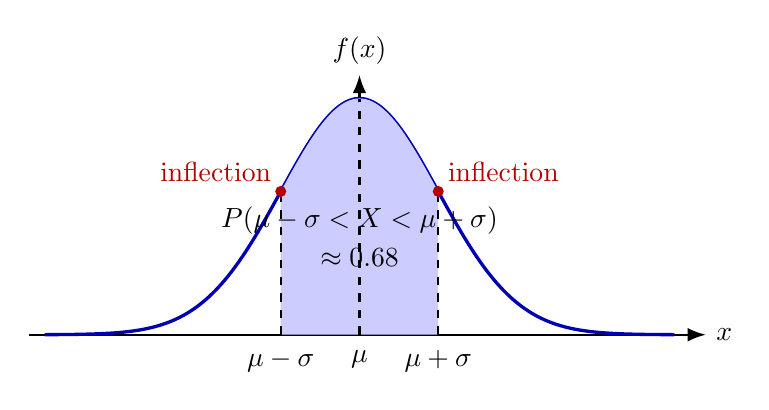
\begin{tikzpicture}[x=1cm,y=1cm,>=Latex]
\draw[->, thick] (-4.2,0) -- (4.4,0) node[right] {$x$};
\draw[->, thick] (0,0) -- (0,3.3) node[above] {$f(x)$};
\draw[very thick, blue!70!black, domain=-4:4, samples=200] plot (\x,{3*exp(-0.5*\x*\x)});
\fill[blue!20, domain=-1:1, samples=150] plot (\x,{3*exp(-0.5*\x*\x)}) -- (1,0) -- (-1,0) -- cycle;
\draw[dashed, thick] (-1,0) -- (-1,{3*exp(-0.5)});
\draw[dashed, thick] (1,0) -- (1,{3*exp(-0.5)});
\draw[dashed, thick] (0,0) -- (0,3);
\node[below] at (-1,-0.08) {$\mu-\sigma$};
\node[below] at (0,-0.08) {$\mu$};
\node[below] at (1,-0.08) {$\mu+\sigma$};
\node[align=center] at (0,1.25) {$P(\mu-\sigma<X<\mu+\sigma)$\\[2pt]$\approx 0.68$};
\fill[red!70!black] (-1,{3*exp(-0.5)}) circle (2pt);
\fill[red!70!black] (1,{3*exp(-0.5)}) circle (2pt);
\node[red!70!black, above left] at (-1,{3*exp(-0.5)}) {inflection};
\node[red!70!black, above right] at (1,{3*exp(-0.5)}) {inflection};
\end{tikzpicture}
\end{document}
